
\section{Interfaz de Usuario y Flujos del Sistema}

El diseño de la interfaz de PANOT se ha construido, como ya se ha comentado, siguiendo las \acrshort{hig} de Apple. La \textit{Jerarquía} visual permite que el 
usuario identifique instantáneamente las acciones críticas, como la captura de voz; la \textit{Armonía} asegura una paleta de colores y tipografías que reducen la 
fatiga visual; y la \textit{Consistencia} garantiza que los patrones de navegación (como la barra de navegación o los botones de ajustes, añadir o aceptar) sean 
familiares para cualquier usuario de la plataforma.

A continuación, se ilustran los flujos de la aplicación siguiendo las Historias de Usuario principales:

\subsubsection{Flujo de Registro de Usuario y Onboarding - \hyperref[req:HU-01]{HU-01}}

\begin{figure}[H]
    \centering
    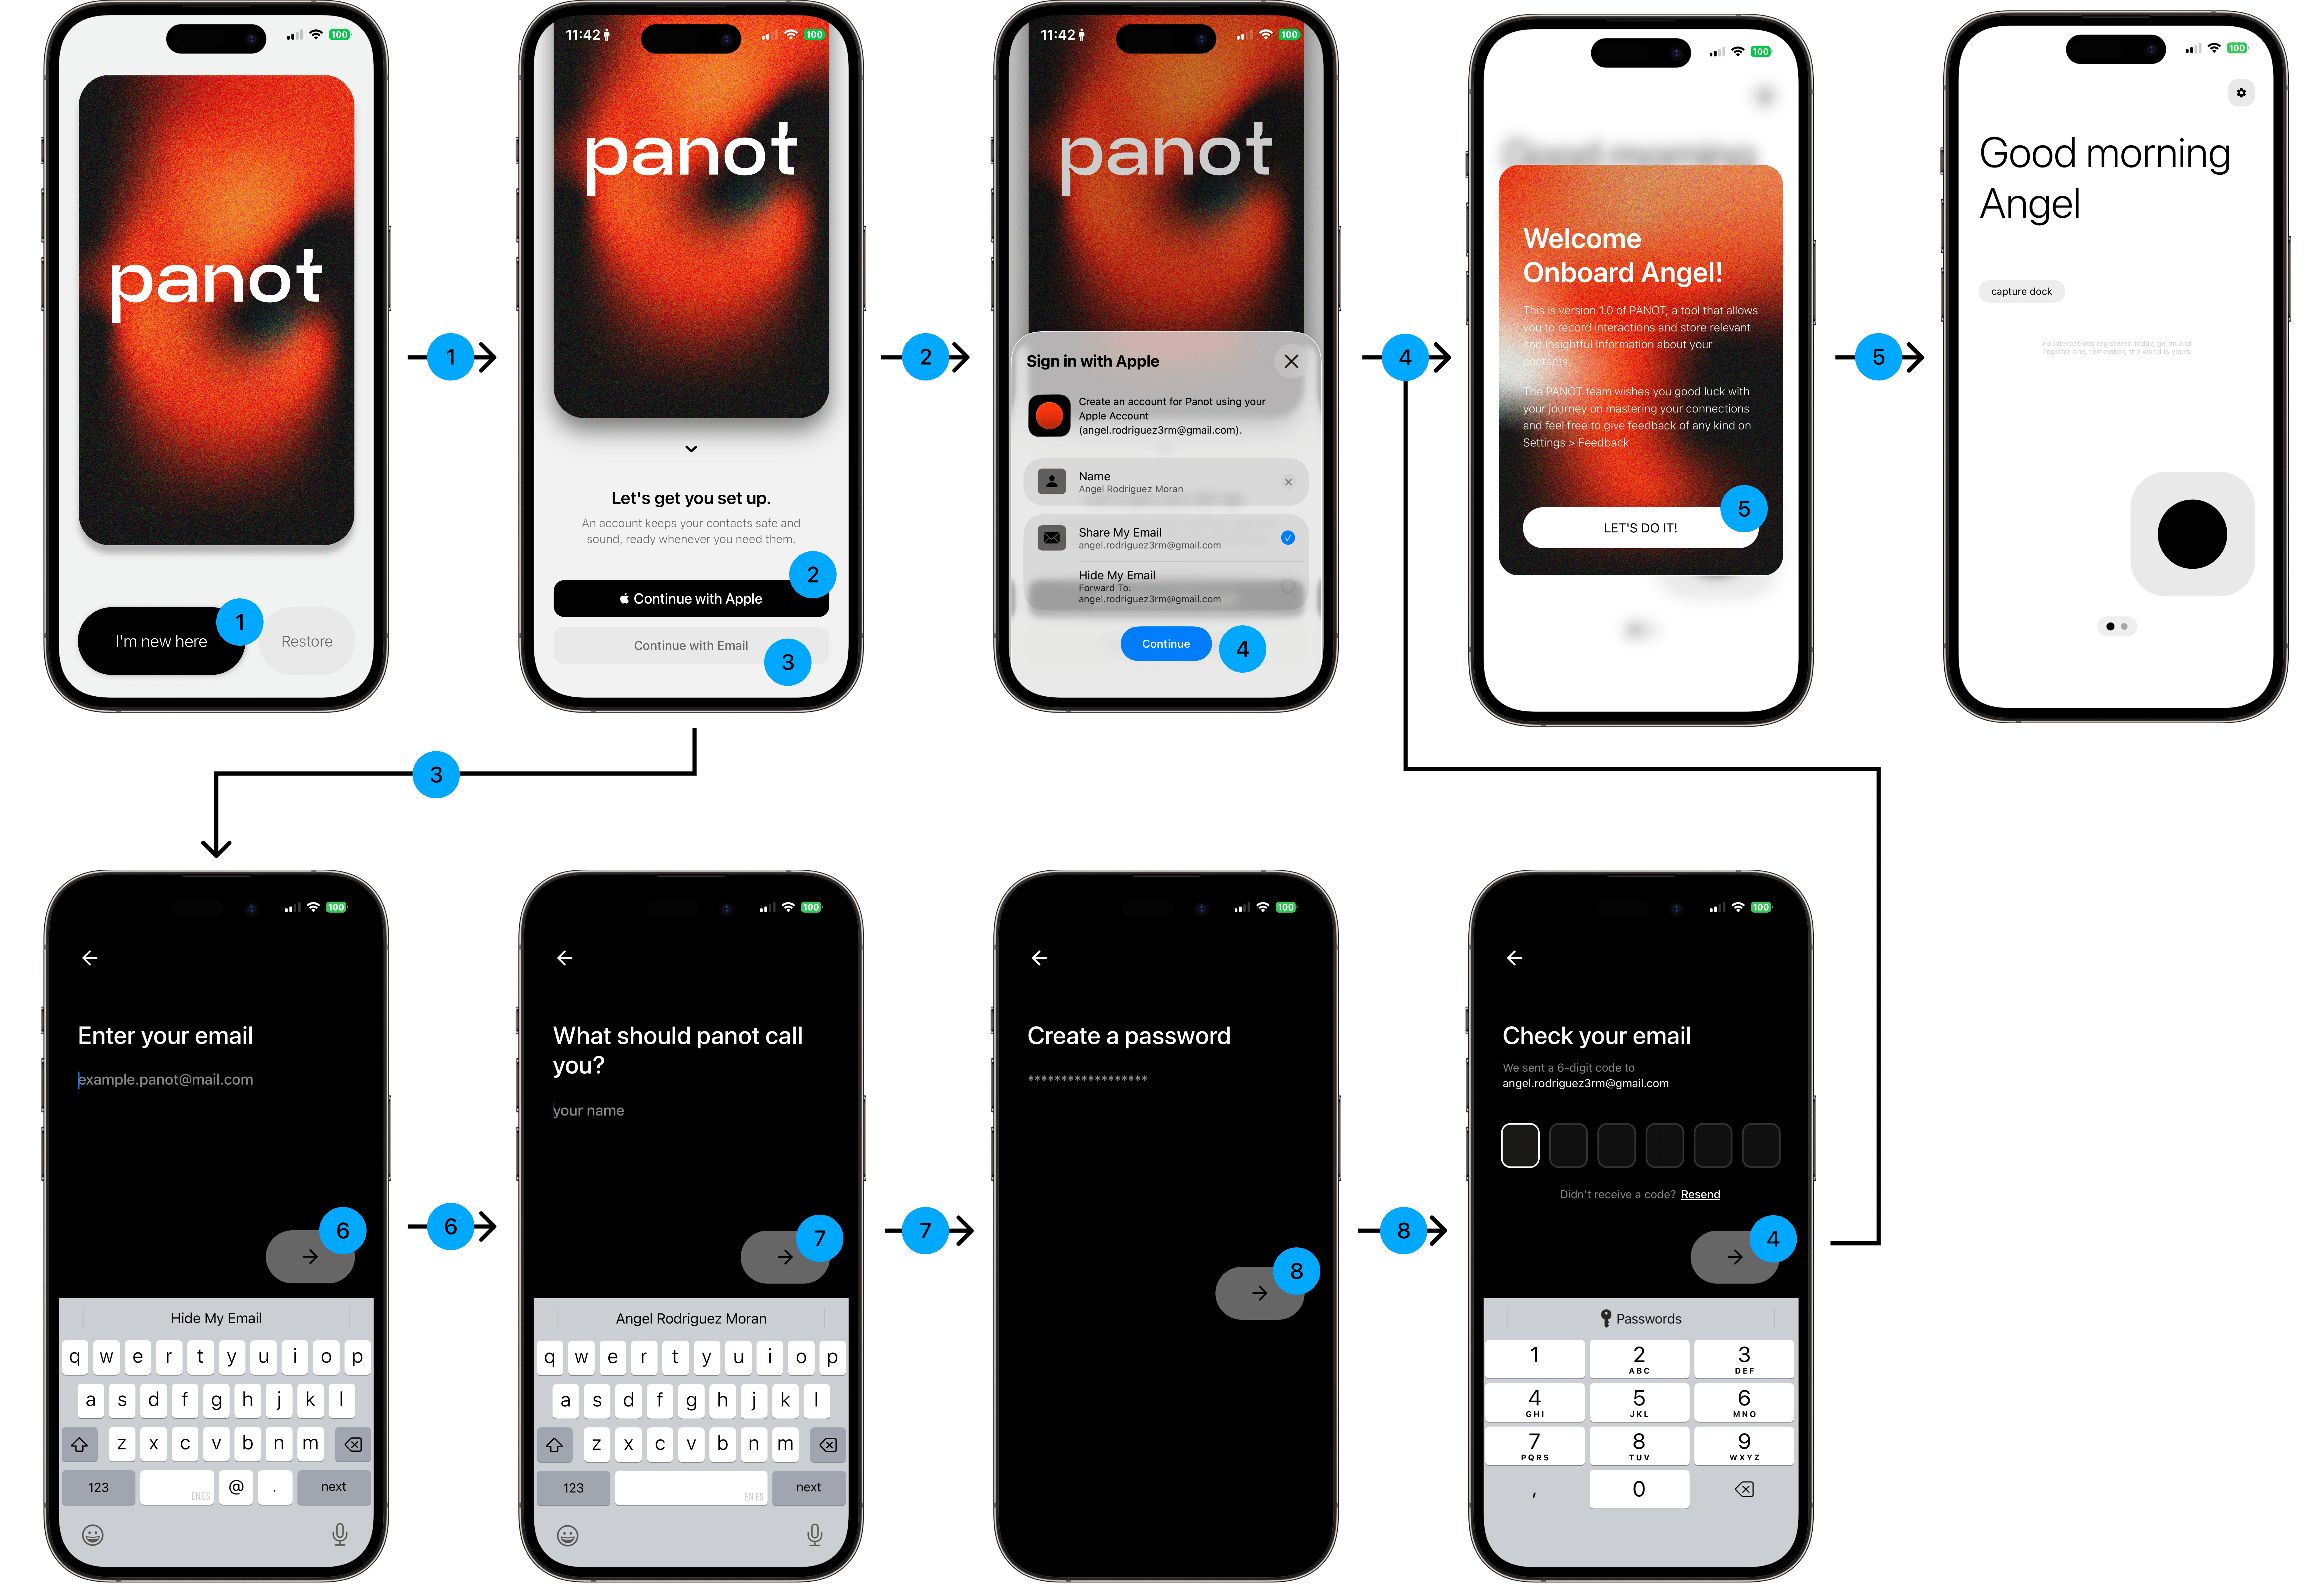
\includegraphics[width=0.8\textwidth]{figures/user-flow-onboarding.png}
    \caption{Flujo de Registro de Usuario y Onboarding}
    \label{fig:onboarding}
\end{figure}

\subsubsection{Flujo de Inicio de Sesión - \hyperref[req:HU-01]{HU-01}}

\begin{figure}[H]
    \centering
    \includegraphics[width=0.75\textwidth]{figures/user-flow-signin.png}
    \caption{Flujo de Inicio de Sesión}
    \label{fig:signin}
\end{figure}

Ambos flujos de Registro \ref{fig:onboarding} e Inicio de Sesión \ref{fig:signin} recogen la posibilidad de que el usuario use su \textit{Correo electrónico} o su \textit{Apple ID} como proveedor de autenticación.

\vspace{3.5cm}
\subsubsection{Flujo de Creación de Contacto - \hyperref[req:HU-02]{HU-02} y \hyperref[req:HU-03]{HU-03}}

El siguiente flujo de ususario abarca las tres posibilidades de creación de un contacto: creación manual (camino \textit{1 - 2 - 4 - 9}), creación con dictado (camino \textit{1 - 2 - 5 - 10 - 11}) e 
importación del contacto (camino \textit{1 - 2 - 6 - 7-  8}).

\begin{figure}[H]
    \centering
    \includegraphics[width=0.8\textwidth]{figures/user-flow-new-contact.png}
    \caption{Flujo de Creación de Contacto}
    \label{fig:new-contact}
\end{figure}

Para validar el funcionamiento de este proceso, se ha analizado la orquestación interna del sistema tras la creación del contacto \textbf{Pedro}. Como se observa en la Figura \ref{fig:trace-pedro}, 
el motor multi-agente inicia una traza de ejecución para crear el nuevo contacto con su grafo contextual correspondiente.

\begin{figure}[H]
    \centering
    \includegraphics[width=0.9\textwidth]{figures/traza-ejemplo-pedro.png}
    \caption{Traza de ejecución en LangSmith para la creación del contacto \textbf{Pedro}.}
    \label{fig:trace-pedro}
\end{figure}

El resultado es el siguiente grafo semántico (ver Figura \ref{fig:grafo-pedro}) donde el contacto no es una entrada tabular, sino el nodo central de una red de conceptos.

\begin{figure}[H]
    \centering
    \includegraphics[width=0.5\textwidth]{figures/grafo-inicial-pedro.png}
    \caption{Grafo de conocimiento resultante de la creación del contacto \textbf{Pedro}.}
    \label{fig:grafo-pedro}
\end{figure}


Posteriormente, al crear el contacto \textbf{Pepe}, el sistema activa el \textit{matching semántico} para identificar nodos comunese entre los contactos. Como se evidencia en la Figura \ref{fig:grafo-pedro-pepe-inicial}, el sistema 
ha identificado de forma autónoma que ambos tienen los nodos comunes \textbf{Universidad Complutense} y \textbf{pádel}, estableciendo una conexión relacional entre los dos contactos sin intervención del usuario.

\begin{figure}[H]
    \centering
    \includegraphics[width=0.8\textwidth]{figures/grafo-pedro-pepe.png}
    \caption{Grafo de conocimiento resultante de la creación del contacto \textbf{Pepe} y la detección de nodos comunes con el contacto \textbf{Pedro}.}
    \label{fig:grafo-pedro-pepe-inicial}
\end{figure}

\vspace{.5cm}
\subsubsection{Flujo de Grabación y Procesamiento de Interacción - \hyperref[req:HU-04]{HU-04}, \hyperref[req:HU-06]{HU-06} y \hyperref[req:HU-08]{HU-08}}

Los siguientes flujos de creación y procesamiento de una interacción que se exponene a continuación corresponden dos variantes: la primera (\hyperref[fig:new-interaction-long]{I}) corresponde a asignación de la interacción a un 
contacto previo a aceptar la creación de la interacción. Mientras que la segunda (\hyperref[fig:new-interaction-short]{II}) corresponde a la creación de una nueva interacción sin asignarla a un contacto previamente.

\begin{figure}[H]
    \centering
    \includegraphics[width=0.8\textwidth]{figures/user-flow-new-interaction-long.png}
    \caption{Flujo de Grabación y Procesamiento de Interacción (I)}
    \label{fig:new-interaction-long}
\end{figure}

\begin{figure}[H]
    \centering
    \includegraphics[width=0.8\textwidth]{figures/user-flow-new-interaction-short.png}
    \caption{Flujo de Grabación y Procesamiento de Interacción (II)}
    \label{fig:new-interaction-short}
\end{figure}

La Figura \ref{fig:grafo-pedro-pepe-nueva-interaccion} muestra el grafo tras procesar las interacciones reflejando la actualización e incorporación 
de los nuevos nodos concepto en ambos contactos.

\vspace{.5cm}
\begin{figure}[H]
    \centering
    \includegraphics[width=0.9\textwidth]{figures/grafo-pedro-pepe-ni.png}
    \caption{Grafo de conocimiento resultante de los contactos \textbf{Pepe} y \textbf{Pedro} tras procesar las nuevas interacciones.}
    \label{fig:grafo-pedro-pepe-nueva-interaccion}
\end{figure}

\newpage
\subsubsection{Flujo de Soporte y Feedback - \hyperref[req:HU-09]{HU-09}}

El siguiente flujo corresponde al envío de un ticket de soporte para un bug (camino \textit{1 - 2 - 4 - 6 - 7}) o una sugerencia (camino \textit{1 - 2 - 3 - 5 - 6 - 7}).

\begin{figure}[H]
    \centering
    \includegraphics[width=0.87\textwidth]{figures/user-flow-support.png}
    \caption{Flujo de Soporte y Feedback}
    \label{fig:support-feedback}
\end{figure}

Para cerrar el ciclo de soporte, se ha verificado la recepción de estos tickets en la base de datos. La Figura \ref{fig:db-tickets} muestra los registros reales en la tabla {\footnotesize \texttt{feedback\_tickets}} de Supabase, 
confirmando que el reporte de errores y sugerencias llega correctamente al equipo de desarrollo para su gestión.

\vspace{.5cm}
\begin{figure}[H]
    \centering
    \includegraphics[width=1\textwidth]{figures/db-feedback-tickets.png}
    \caption{Verificación de persistencia: Filas de la base de datos con los tickets de soporte enviados.}
    \label{fig:db-tickets}
\end{figure}

\subsubsection{Flujo de Configuración y Ajustes}

\begin{figure}[H]
    \centering
    \includegraphics[width=0.8\textwidth]{figures/user-flow-settings.png}
    \caption{Flujo de Configuración y Ajustes}
    \label{fig:configuracion-ajustes}
\end{figure}